\section{Task 3: Principal Component Analysis (by Jan)}

\subsection{Preceding tasks}
Firstly i need to read the csv file in a compatible format. I choose pandas dataframes as it is easy to use and i am already used to it form the other courses. I read the csv via:

\begin{verbatim}
df = pd.read_csv("../Wine_Test_01.csv")
\end{verbatim}
Next i print the dataset as shown in \autoref{fig:dataset}:

\begin{figure}[H]
\centerline{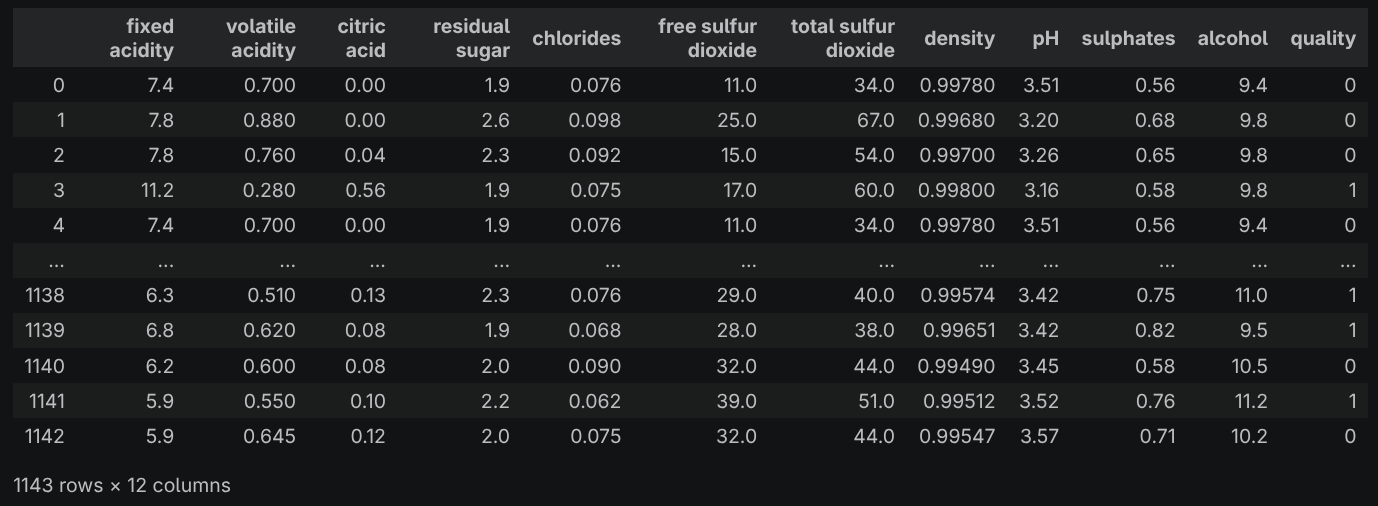
\includegraphics[width=\textwidth]{Images/1779112013.png}}
\caption{Wine test dataset in Pandas}
\label{fig:dataset}
\end{figure}

\subsection{Task a)}

\subsubsection{Required libraries}

For the preceding task i firstly imported the required libraries to run the program. When and why the libraries are used will be explained later:

\begin{verbatim}
import pandas as pd
from sklearn.preprocessing import StandardScaler
from sklearn.decomposition import PCA
import matplotlib.pyplot as plt
import numpy as np
\end{verbatim}

\subsubsection{Scale dataset}

Before performing PCA the dataset needs to be scaled as with all machine learning tasks. In this case i use the StandardScaler from sklearn preprocessing as it is normally used for such tasks:

\begin{verbatim}
scaler = StandardScaler()
y = df["quality"]
X = df.drop(columns=["quality"])
X = scaler.fit_transform(df)
X
\end{verbatim}

\subsubsection{Perform PCA on all attributes and get cumulative variance}

Next i perform PCA on all attributes as stated in the task description. For that i use the PCA library from sklearn decomposition. With this library to perform a PCA on all attributes you just don't provide the \verb|n_components| variable:

\begin{verbatim}
pca = PCA()
pca.fit(X)
\end{verbatim}
After that i get the \verb|explained_variance_ration_| and calculate the cumulative variance via \verb|np.cumsum| from it:

\begin{verbatim}
cum_cov = np.cumsum(cov)
\end{verbatim}
This results in following array with the cumulative variances:
\begin{verbatim}
array([0.26347428, 0.44561281, 0.58392261, 0.68498203, 0.76667449,
    0.82351255, 0.87537205, 0.91853493, 0.9534041 , 0.98054548,
    0.99512954, 1.        ])
\end{verbatim}

\subsubsection{Plot results}

Lastly as asked in the task description i print the result like we did in class. For this i use matplotlib and following config:

\begin{verbatim}
plt.plot(cum_cov)
plt.xlabel("Number of components")
plt.ylabel("Cumulative variance")
plt.show()
\end{verbatim}
which leads to output in \autoref{fig:var_plot}:

\begin{figure}[H]
\centerline{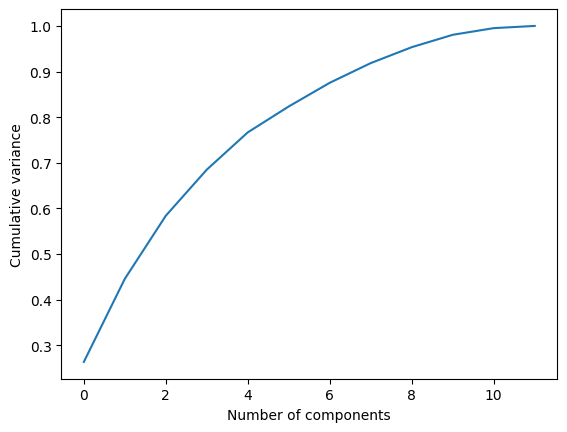
\includegraphics[width=\textwidth]{Images/Task3_plot.png}}
\caption{"Number of components" vs "Cumulative variance" plot result}
\label{fig:var_plot}
\end{figure}
This plot corresponds with the plot we did in class.

\subsubsection{Choose principal components}

Lastly we should decide with how many principal components we should proceed. As the cumulative variance should be over 90\% i wrote i small loop to dynamically choose the principal components:

\begin{verbatim}
for index, value in enumerate(cum_cov):
    if value >= 0.9:
        p_c = index + 1
        break
\end{verbatim}
The result was that in on this dataset we should use \textbf{8 principal componenets}. After that i used the \verb|p_c| variable to generate a new reduced dataset via PCA for Task 3 b):

\begin{verbatim}
pca = PCA(n_components=p_c)
X_PCA = pca.fit_transform(X)
\end{verbatim}

\subsection{Task b)}

With Task 3 b) we should implement the PCA in the Task 1 c) and train and the model with the reduced number of components. For this i used the code provided by Maria in Task 1 c) with some slight modifications.

\subsubsection{Required Libraries}

First i needed to include the required libraries in my jupyter notebook to run the given code:

\begin{verbatim}
from sklearn.model_selection import train_test_split, GridSearchCV
from sklearn.preprocessing import StandardScaler
from sklearn.pipeline import Pipeline
from sklearn.svm import SVC
from sklearn.decomposition import PCA
\end{verbatim}

\subsubsection{Implementing PCA}

After that i could modify marias code to implement PCA. As marias code already implemented a \verb|StandardScaler| there was no need to do this separately/again. With this problem already fixed i only needed to add following lines:

\begin{verbatim}
pipe = Pipeline([
    ("scaler", StandardScaler()),
    ("pca", PCA()),     # Implemented PCA
    ("svm",    SVC()),
])
\end{verbatim}
Firstly this line to add PCA to the pipeline. Here the order is important as the PCA needs to be performed after the StandardScaler and before the SVM.

\begin{verbatim}
param_grid = {
    "pca__n_components": [p_c],     # Added PCA components variable
    "svm__kernel": ["linear", "rbf"],
    "svm__C":      [0.1, 1, 10, 100, 1000],
    "svm__gamma":  [1, 0.1, 0.01, 0.001, 0.0001],
}
\end{verbatim}
And secondly this line to fix the PCA-components to the in the previous task discovered value which should be 8.

\subsubsection{Results}

Finally althrough this model has been trained and tested with a reduced set of compoenets via PCA the results are similar as with training and testing the model with the full 11 attributes:

\begin{verbatim}
Running 10 train/test runs with GridSearch (may take ~1 min)

Run  1  accuracy = 0.7817  best params = {'pca__n_components': 8,
'svm__C': 1, 'svm__gamma': 0.1, 'svm__kernel': 'rbf'}

Run  2  accuracy = 0.7773  best params = {'pca__n_components': 8,
'svm__C': 1000, 'svm__gamma': 0.01, 'svm__kernel': 'rbf'}

Run  3  accuracy = 0.7686  best params = {'pca__n_components': 8,
'svm__C': 1000, 'svm__gamma': 0.01, 'svm__kernel': 'rbf'}

Run  4  accuracy = 0.7642  best params = {'pca__n_components': 8,
'svm__C': 1, 'svm__gamma': 0.01, 'svm__kernel': 'rbf'}

Run  5  accuracy = 0.7249  best params = {'pca__n_components': 8,
'svm__C': 1, 'svm__gamma': 0.1, 'svm__kernel': 'rbf'}

Run  6  accuracy = 0.7249  best params = {'pca__n_components': 8,
'svm__C': 10, 'svm__gamma': 0.1, 'svm__kernel': 'rbf'}

Run  7  accuracy = 0.8035  best params = {'pca__n_components': 8,
'svm__C': 1, 'svm__gamma': 0.1, 'svm__kernel': 'rbf'}

Run  8  accuracy = 0.7642  best params = {'pca__n_components': 8,
'svm__C': 1000, 'svm__gamma': 0.01, 'svm__kernel': 'rbf'}

Run  9  accuracy = 0.7642  best params = {'pca__n_components': 8,
'svm__C': 1000, 'svm__gamma': 0.01, 'svm__kernel': 'rbf'}

Run 10  accuracy = 0.7249  best params = {'pca__n_components': 8,
'svm__C': 100, 'svm__gamma': 0.01, 'svm__kernel': 'rbf'}

============================================================
Task 1c summary over 10 runs
  Mean accuracy: 0.7598
  Std  accuracy: 0.0255
============================================================
\end{verbatim}
